\begin{figure}
	\centering
	\begin{subfigure}[b]{.58\textwidth}
		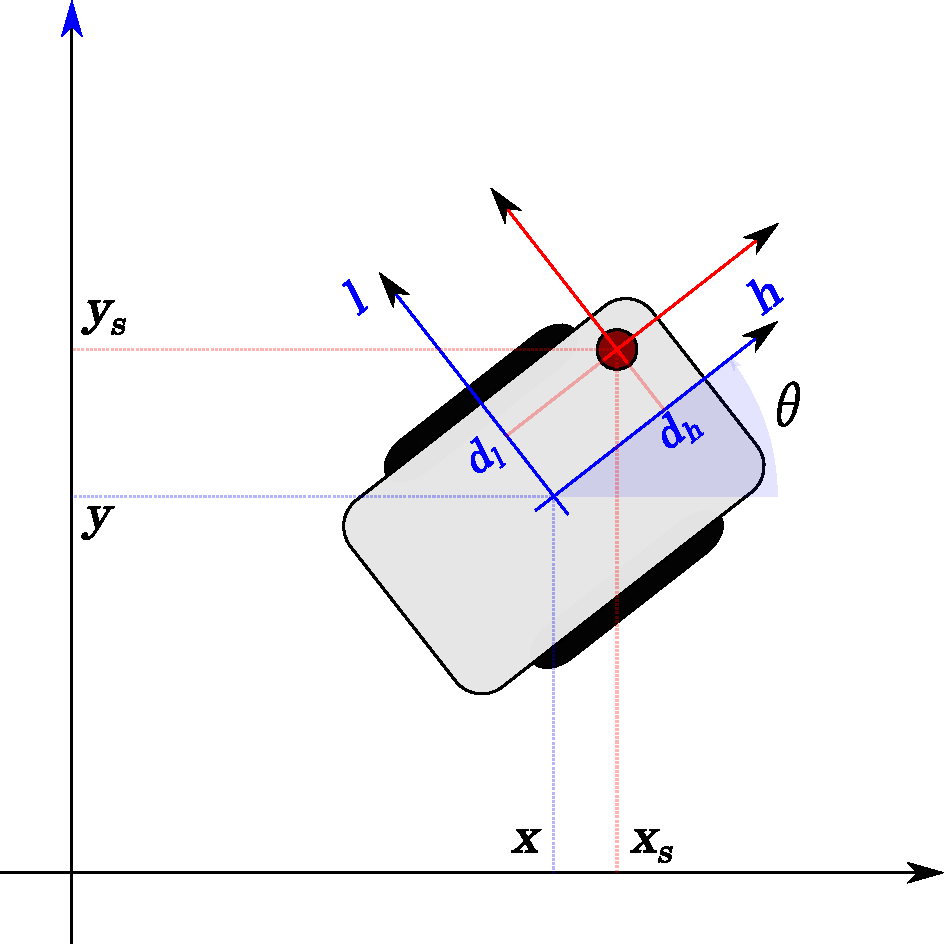
\includegraphics[width=\linewidth]{./img/frames_of_reference.pdf}
		\caption{The \emph{sensor} \FoR{}, inside the \emph{robot} \FoR{}, inside the \emph{map} \FoR{}.}
		\label{fig.fors.nested}
	\end{subfigure}
	\hfill
	\begin{subfigure}[b]{.38\textwidth}
		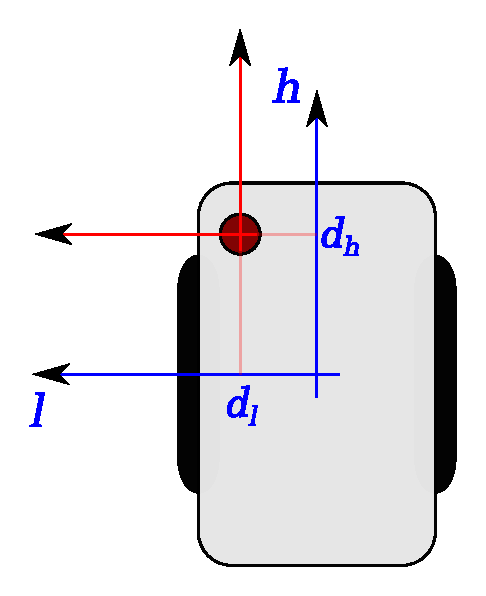
\includegraphics[width=\linewidth]{./img/robot_for.pdf}
		\caption{The \emph{robot} \FoR{} and the sensor position within it.}
		\label{fig.fors.robot}
	\end{subfigure}
	\caption{Frames of references (\FoR) considered the SLAM problem.}
	\label{fig.fors}
\end{figure}

It is important to understand that several Frames of Reference (\FoR{}) are involved in \SLAM{} (as shown in Figure \ref{fig.fors}):
\begin{itemize}
	\item The \emph{map} (or \emph{global}) \FoR{}, \ie{} the one used for representing the map and the current robot orientation and position. 
	It is arbitrary.
	
	\item The \emph{robot} (or \emph{local}) \FoR{}, \ie{} the one defined according to the reference center of the robot. 
	For what concerns this report, we consider a frame having its origin into the robot geometry center, the abscissas axis always coinciding with the heading direction, and the ordinate axis coinciding with the lateral direction (increasing on the left, as shown in Figure \ref{fig.fors.robot}).
	
	\item The \emph{sensor} (or \emph{measurement}) \FoR{}, which depends on the exteroceptive sensor position within the robot frame, and is in general different from the robot frame. 
	E.g., the sensor may be in position $(d_h,\, d_l)^\top$ w.r.t. the robot frame, as shown in Figure \ref{fig.fors.robot}, and this translation should be taken into account when handling sensor data in order to understand obstacles position on the map.
	In this tutorial we consider, for simplicity, the sensor frame to be coincident with the robot frame \ie{} $d_h = d_h = 0$.
	
\end{itemize}

Since part of the SLAM process is to build a map of the environment under the hypothesis that the robot has no prior knowledge about it, there is no constraint on how the robot should choose the initial global frame.
In what follows, we (and the robot) assume that the global frame coincides with the initial robot frame, \ie{} the map frame is defined by the initial pose of the robot into the environment: the origin is its \emph{very first} position, the abscissas axis is its \emph{initial} heading direction and, consequently, the ordinate axis is its \emph{initial} lateral direction.

\subsection{The motion model}
	The motion model is a function $g : \mathbb{R}^n \times \mathbb{R}^m \rightarrow \mathbb{R}^n$ mapping the previous robot pose vector, $\vect{r}_{t-1} \in \mathbb{R}^n$, \ie{} the vector containing the robot position and orientation (which are relative to the \emph{map} frame), into the current one, $\vect{r}_t \in \mathbb{R}^n$, by taking into account the last \emph{control} vector $\vect{u}_t \in \mathbb{R}^m$, \ie{} the vector containing proprioceptive data (which is relative to the \emph{robot} frame). 
	More formally:
	\[
		\vect{r}_t = g(\vect{r}_{t-1},\, \vect{u}_t)
	\]
	
	The motion model aims to keep track the robot movements in order to provide an updated estimation of its pose vector.
	
	\paragraph{Example: Differential robot on the plane.}
		Suppose we only own a two-wheeled, differential robot having no odometric sensor, which is often the case in experimental setups.
		The distance between the wheels is $2L$.
		Suppose we want to experiment the SLAM problem on planar arena containing some obstacles.
		Finally, suppose that each step of the robot controller is executed after ${\Delta T}_t$ seconds since the end of the previous step and that the duration of each step is negligible.
		Under such assumptions, movements relative to the $z$-axis are not so relevant: we are only interested in the robot to solve the SLAM problem on the 2D plane.
		In this setting we can assume the robot pose vector to be the triplet $\vect{r}_t = (x_t,\, y_t,\, \theta_t)^\top$, \ie{} the position and bearing of the robot w.r.t. the global frame, and the control vector to be the triplet $\vect{u}_t = (v_{l,t},\, v_{r,t},\, {\Delta T}_t)^\top$, \ie{} the velocities imposed to the wheels actuators at the end of the previous control step and the time elapsed since that moment.
		Notice that, if we assume ${\Delta T}_t$ to be constant, the control vector is the pair $\vect{u}_t = (v_{l,t},\, v_{r,t})^\top$.
		Under such hypotheses, the motion model could be defined as follows\footnote{\label{sec.models.alert}\notationAlert}:
		\begin{equation}
			\label{eq.motion.differential}
			\left(\begin{array}{c}
				x \\ y \\ \theta
			\end{array}\right)
			\leftarrow
			\left(\begin{array}{ccc}
				\cos{\theta} & -\sin{\theta} & 0 \\
				\sin{\theta} & \cos{\theta} & 0 \\
				0 & 0 & 1
			\end{array}\right)
			\cdot {\Delta T} \cdot I \cdot
			\left(\begin{array}{c}
				\frac{v_l + v_r}{2} \\ 
				0 \\
				\frac{v_r - v_l}{2L}
			\end{array}\right)
			+
			\left(\begin{array}{c}
				x \\ y \\ \theta
			\end{array}\right)
		\end{equation}
		where ${\Delta T} \cdot I$ is a diagonal $3 \times 3$ matrix having each element on the diagonal equal to ${\Delta T}$.
		Equation \ref{eq.motion.differential} computes the translation and rotation the robot performed within its reference frame during the last control step as a function of the velocity imposed to the wheels. 
		Such values are converted into the map frame and added to the previous position and orientation in order to achieve the new ones. 
		
		Please consider reading Appendix \ref{app.affine2d} and \ref{app.differential_drive} in order to recall conversions between reference frames and differential drive.
		
	\paragraph{Example: Robot equipped with odometric sensor on the plane.}
		Suppose our robot is embodied with an odometric sensor, which periodically provides a triplet $(dh,\, dl, d\theta)^\top$, \ie{} the variations in the heading and lateral directions and the angular variation since the last update. 
		Such variations are of course relative to the robot frame.
		We assume such a sensor frequency to be high.
		In this case the motion model could be simply defined as follows\footnoteref{sec.models.alert}:
		\begin{equation}
			\label{eq.motion.odometrix}
			\left(\begin{array}{c}
				x \\ y \\ \theta
			\end{array}\right)
			\leftarrow
			\left(\begin{array}{ccc}
				\cos{\theta} & -\sin{\theta} & 0 \\
				\sin{\theta} & \cos{\theta} & 0 \\
				0 & 0 & 1
			\end{array}\right)
			\cdot
			\left(\begin{array}{c}
				dh \\
				dl \\
				d\theta
			\end{array}\right)
			+
			\left(\begin{array}{c}
				x \\ y \\ \theta
			\end{array}\right)
		\end{equation}
		This means the variations relative to the robot frame are simply converted into the map frame.
		
		\begin{important}
			Always take care of normalizing the angle $\theta + d\theta$, since it's a sum of angles.
		\end{important}

\subsection{The inverse observation model}
	The inverse observation model is a function $\eta : \mathbb{R}^n \times \mathbb{R}^p \rightarrow \mathbb{R}^q$ mapping a measurement vector, $\vect{s}_{t} \in \mathbb{R}^p$, \ie{} the vector containing the data identifying an obstacle from the exteroceptive sensor (w.r.t. the \emph{sensor} frame), into the position vector, $\vect{m}_{t} \in \mathbb{R}^q$, of the corresponding landmark (which is relative to the \emph{global} frame), by taking into account the current \emph{robot} pose vector $\vect{r}_t \in \mathbb{R}^n$.
	More formally:
	\[
		\vect{m}_t = \eta(\vect{r}_{t},\, \vect{s}_t)
	\]
	
	The inverse observation model aims to produce an estimation of the position vector for some maybe-unknown landmark taking into account the measurement vector received by the exteroceptive sensor and the current estimation of the robot pose.
	Such estimation is compared with the known landmarks positions in order to understand if it is relative to one of them.
	
	\paragraph{Example: Laser scanner on top of a robot.}
		Suppose a laser scanner is located in position $(d_h,\,d_l)^\top$ within the robot frame\footnote{coordinates are expressed w.r.t. the $h$eading and $l$ateral axes}.
		In the real case, the sensor will probably be on the top of the robot.
		The laser scanners usually provide distance and angle (w.r.t. the sensor frame) for each obstacle which is closer than a maximum distance $D_{max} > 0$.
		Moreover, they are usually characterized by $W_{V},W_{H} \subseteq [\,-\pi,\, \pi\,]$: vertical and horizontal angle windows, respectively.
		Using spheric coordinates, $\rho$, $\theta$ and $\phi$, we say that the sensor can only perceive obstacles such that $\rho \leq D_{max}$ and $\theta \in W_{H}$ and $\phi \in W_{V}$.
		For what concerns this example, we suppose that $W_H = (\,-\pi,\, \pi\,]$ and $W_V = \{\, \pi / 2 \,\}$, \ie{} the robot can perceive obstacles in any direction on the horizontal plane.
		In the real case, one may take into account that the sensor be in an higher position than the robot and therefore not being able to perceive shorter obstacles.
		
		Under such hypotheses\footnote{\label{sec.models.subscript}the subscript indicating the computational step is omitted in order to keep the notation readable}, the measurement vector is the distance-and-angle pair $\vect{s} = (\rho,\, \alpha)^\top$, the landmark position is the pair $\vect{m} = (x_m,\, y_m)^\top$, and the inverse observation model can be simply defined as follows:
		\begin{equation}
			\label{eq.inv_observation.laser}
			\left(\begin{array}{c}
				x_m \\ y_m
			\end{array}\right)
			=
			\left(\begin{array}{ccc}
				\cos{\theta} & -\sin{\theta} \\
				\sin{\theta} & \cos{\theta}
			\end{array}\right)
			\cdot
			\left(
				\left(\begin{array}{c}
					d_x \\ d_y
				\end{array}\right)
				+ \rho \cdot
				\left(\begin{array}{cc}
					\cos{\alpha} & -\sin{\alpha} \\
					\sin{\alpha} & \cos{\alpha}
				\end{array}\right)
			\right)
			+
			\left(\begin{array}{c}
				x \\ y
			\end{array}\right)
		\end{equation}
		
		Please note that, if $d_x = d_y = 0$, \ie{} sensor is located into the robot center, Equation \ref{eq.inv_observation.laser} can reduces to:
		\[
			\left(\begin{array}{c}
				x_m \\ y_m
			\end{array}\right)
			=
			\rho \cdot
			\left(\begin{array}{ccc}
				\cos{(\theta + \alpha)} & -\sin{(\theta + \alpha)} \\
				\sin{(\theta + \alpha)} & \cos{(\theta + \alpha)}
			\end{array}\right)
			+
			\left(\begin{array}{c}
				x \\ y
			\end{array}\right)
		\]
		
		\begin{figure}
			\centering
			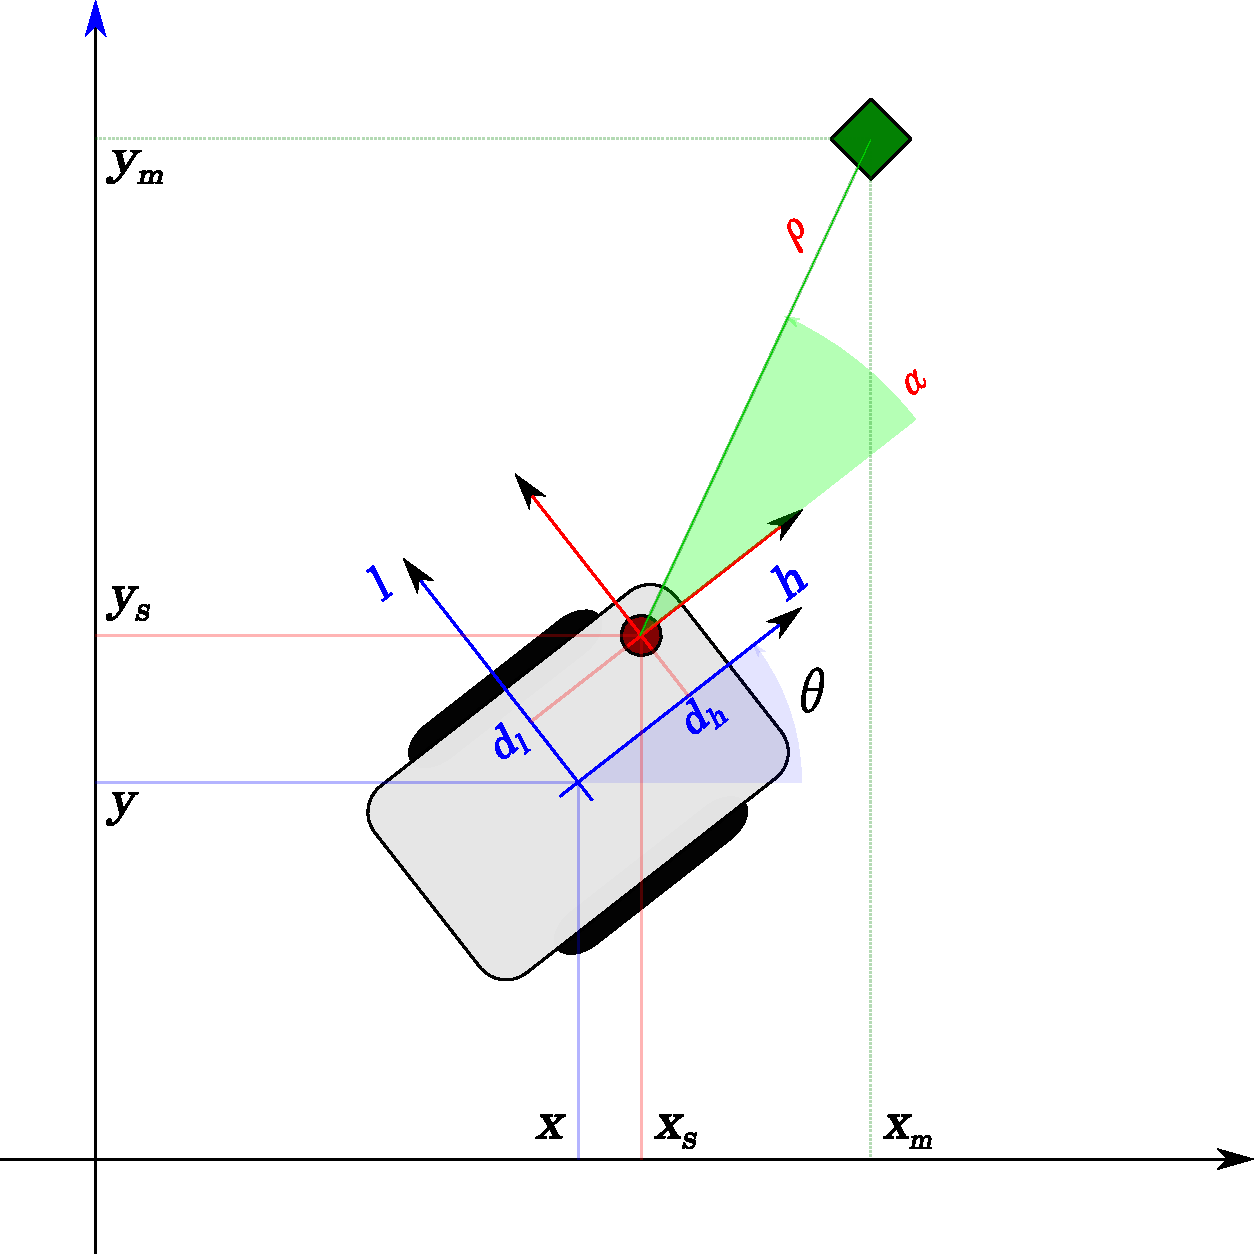
\includegraphics[width=0.5\textwidth]{./img/observation.pdf}
			\caption{Direct and inverse observation on the 2D plane.}
			\label{fig.observation}
		\end{figure}
		
\subsection{The (direct) observation model}
	The observation model is a function $h : \mathbb{R}^n \times \mathbb{R}^q \rightarrow \mathbb{R}^p$ mapping the position vector $\vect{m}_t \in \mathbb{R}^q$ of some landmark (which is relative to the \emph{global} frame), into the measurement vector, $\vect{s}_{t} \in \mathbb{R}^p$, (w.r.t. the \emph{sensor} frame) expected for that landmark. 
	It takes into account the current \emph{robot} pose vector $\vect{r}_t \in \mathbb{R}^n$.
	More formally:
	\[
		\vect{s}_t = h(\vect{r}_{t},\, \vect{m}_t)
	\]
	
	The observation model aims to produce an estimation of the measurement vector for some known landmark taking into account the current estimation of the robot pose vector and the landmark position vector. 
	Such estimation is compared with the actual measurement vector relative to the recognized landmark and their difference is used to reduce the current uncertainty about the robot pose. 
	
	\paragraph{Example: Laser scanner on top of a robot.}
		Here we consider the same hypotheses of the previous example\footnoteref{sec.models.subscript}.
		Let $(x_s,\, x_s)^\top$ be the position of the sensor w.r.t. the \emph{global} frame: the same position is $(d_h,\, d_l)^\top$ within the \emph{robot} frame.
		The equation relating the two coordinate frames is the following:
		\begin{equation}
			\left(\begin{array}{c}
				x_s \\ y_s
			\end{array}\right)
			=
			\left(\begin{array}{ccc}
				\cos{\theta} & -\sin{\theta} \\
				\sin{\theta} & \cos{\theta}
			\end{array}\right)
			\cdot
			\left(\begin{array}{c}
				d_h \\ d_l
			\end{array}\right)
			+
			\left(\begin{array}{c}
				x \\ y
			\end{array}\right)
		\end{equation}
		Notice that $(x_s,\, y_s)^\top$ is the origin of the \emph{sensor} frame and that the measurement vector $\vect{s} = (\rho,\, \alpha)^\top$ consists of the polar coordinates of the landmark position $\vect{m} = (x_m,\, y_m)^\top$ according to such frame.
		So, the observation model is simply:
		\[
			\left(\begin{array}{c}
				\rho \\ \alpha
			\end{array}\right)
			=
			\left(\begin{array}{ccc}
				\sqrt{(x_m - x_s)^2 + (y_m - y_s)^2} \\
				\mathrm{atan2}(y_m - y_s,\ x_m - x_s) - \theta
			\end{array}\right)
		\]
		where $x_s$ and $y_s$ are both functions of $x$, $y$ and $\theta$.
		
		Please note that, if $d_x = d_y = 0$, then $(x_s,\, y_s)^\top \equiv (x,\, y)^\top$, so the motion model reduces to: 
		\[
			\left(\begin{array}{c}
				\rho \\ \alpha
			\end{array}\right)
			=
			\left(\begin{array}{ccc}
				\sqrt{(x_m - x)^2 + (y_m - y)^2} \\
				\mathrm{atan2}(y_m - y,\ x_m - x) - \theta
			\end{array}\right)
		\]
		which is indeeds a far simpler expression.
		
		\begin{important}
			Always take care of normalizing the angle $\alpha$, since it's a subtraction of angles.
		\end{important}